\section{Telescope}
\label{sec:Telescope}

The layout of the Timepix3 telescope is shown in Fig. \ref{fig:Telescope}, where the coordinate system is defined such that the $z$ axis corresponds to the beam direction, the $x$ axis is horizontal, and the $y$ axis is vertical.
The telescope is made of two separate arms, located downstream and upstream of a Device Under Test (DUT). Each arm consists of four planes, which are separated by $25$~mm and rotated of $9^\circ$ around the $x$ and $y$ axes in order to improve the single hit resolution. The planes are equipped with a matrix of $256 \times 256$ hybrid pixel detector readout chips, the Timepix3 ASICs, bump bonded to p-in-n silicon sensors of $300~\mu$m thickness and $55~\mu$m pitch, resulting in a total active area of $14.080 \times 14.080$~mm$^2$ per plane. Each plane has a material budget in units of radiation length of $x/X_0 = 2.6\%$.
The whole telescope can be shifted along the $x$ and $y$ axes, in order to move it out of the beam without the need to physically access the experimental area.
Each arm can be shifted along the $y$ and $z$ axes, thus allowing the separation between the two arms to be adapted to the size of the DUT. The latter is mounted on an automatic stage, which allows shifts along the $x$ and $y$ axes with a precision of $1~\mu$m, as well as rotations around the $y$ axis with a precision of $0.01^\circ$. In addition, each plane can be shifted independently of the others along the $z$ axis.

Each telescope plane is read out by half a Speedy PIxel Detector Readout (SPIDR) board, a readout system developed at NIKHEF, implemented in FPGA and connected to a $10$~GBit Ethernet link.

Two scintillators are positioned at the two edges of the telescope and allow to trigger the data acquisition of the DUT based on the presence of incoming particles.
No trigger signal is required to start the data acquisition of the telescope planes, since the Timepix3 ASIC has a data driven readout mode, which sends out a data packet with hit coordinates, Time over Threshold (ToT), and Time of Arrival (ToA), as soon as a hit is processed.
The ToT is related to the charge deposited by the incoming particle, while the ToA allows to match clusters on different planes and hence reconstruct tracks, as well as to associate the reconstructed tracks with the corresponding clusters on the DUT.
In order to facilitate the synchronisation between telescope and DUT, the trigger signal is sent to the telescope too.
In addition, a busy signal is sent from the DUT to the telescope, in order to inhibit the generation of further trigger signals while the DUT is reading out an event. This ensure that the DUT and the telescope record exactly the same number of trigger signals.

Both the Beetle and Timepix3 ASICs have an internal clock of $40$~MHz.
The phase between these internal clocks and the trigger signal is measured by a Time to Digital Converter (TDC) with a timing resolution of $?$~ns.

The telescope can cope with a hit rate of $40$~MHz cm$^{-2}$ s$^{-1}$ and provides a pointing precision at the DUT of $1.54 \pm 0.11~\mu$m and a timing resolution of $1.56$~ns. 

A clustering algorithm is applied to reconstruct clusters out of neighbouring hits on each telescope plane. The cluster position is calculated as the center of gravity of the hit positions, weighted by the corresponding ToTs.

\begin{figure}[]
\centering
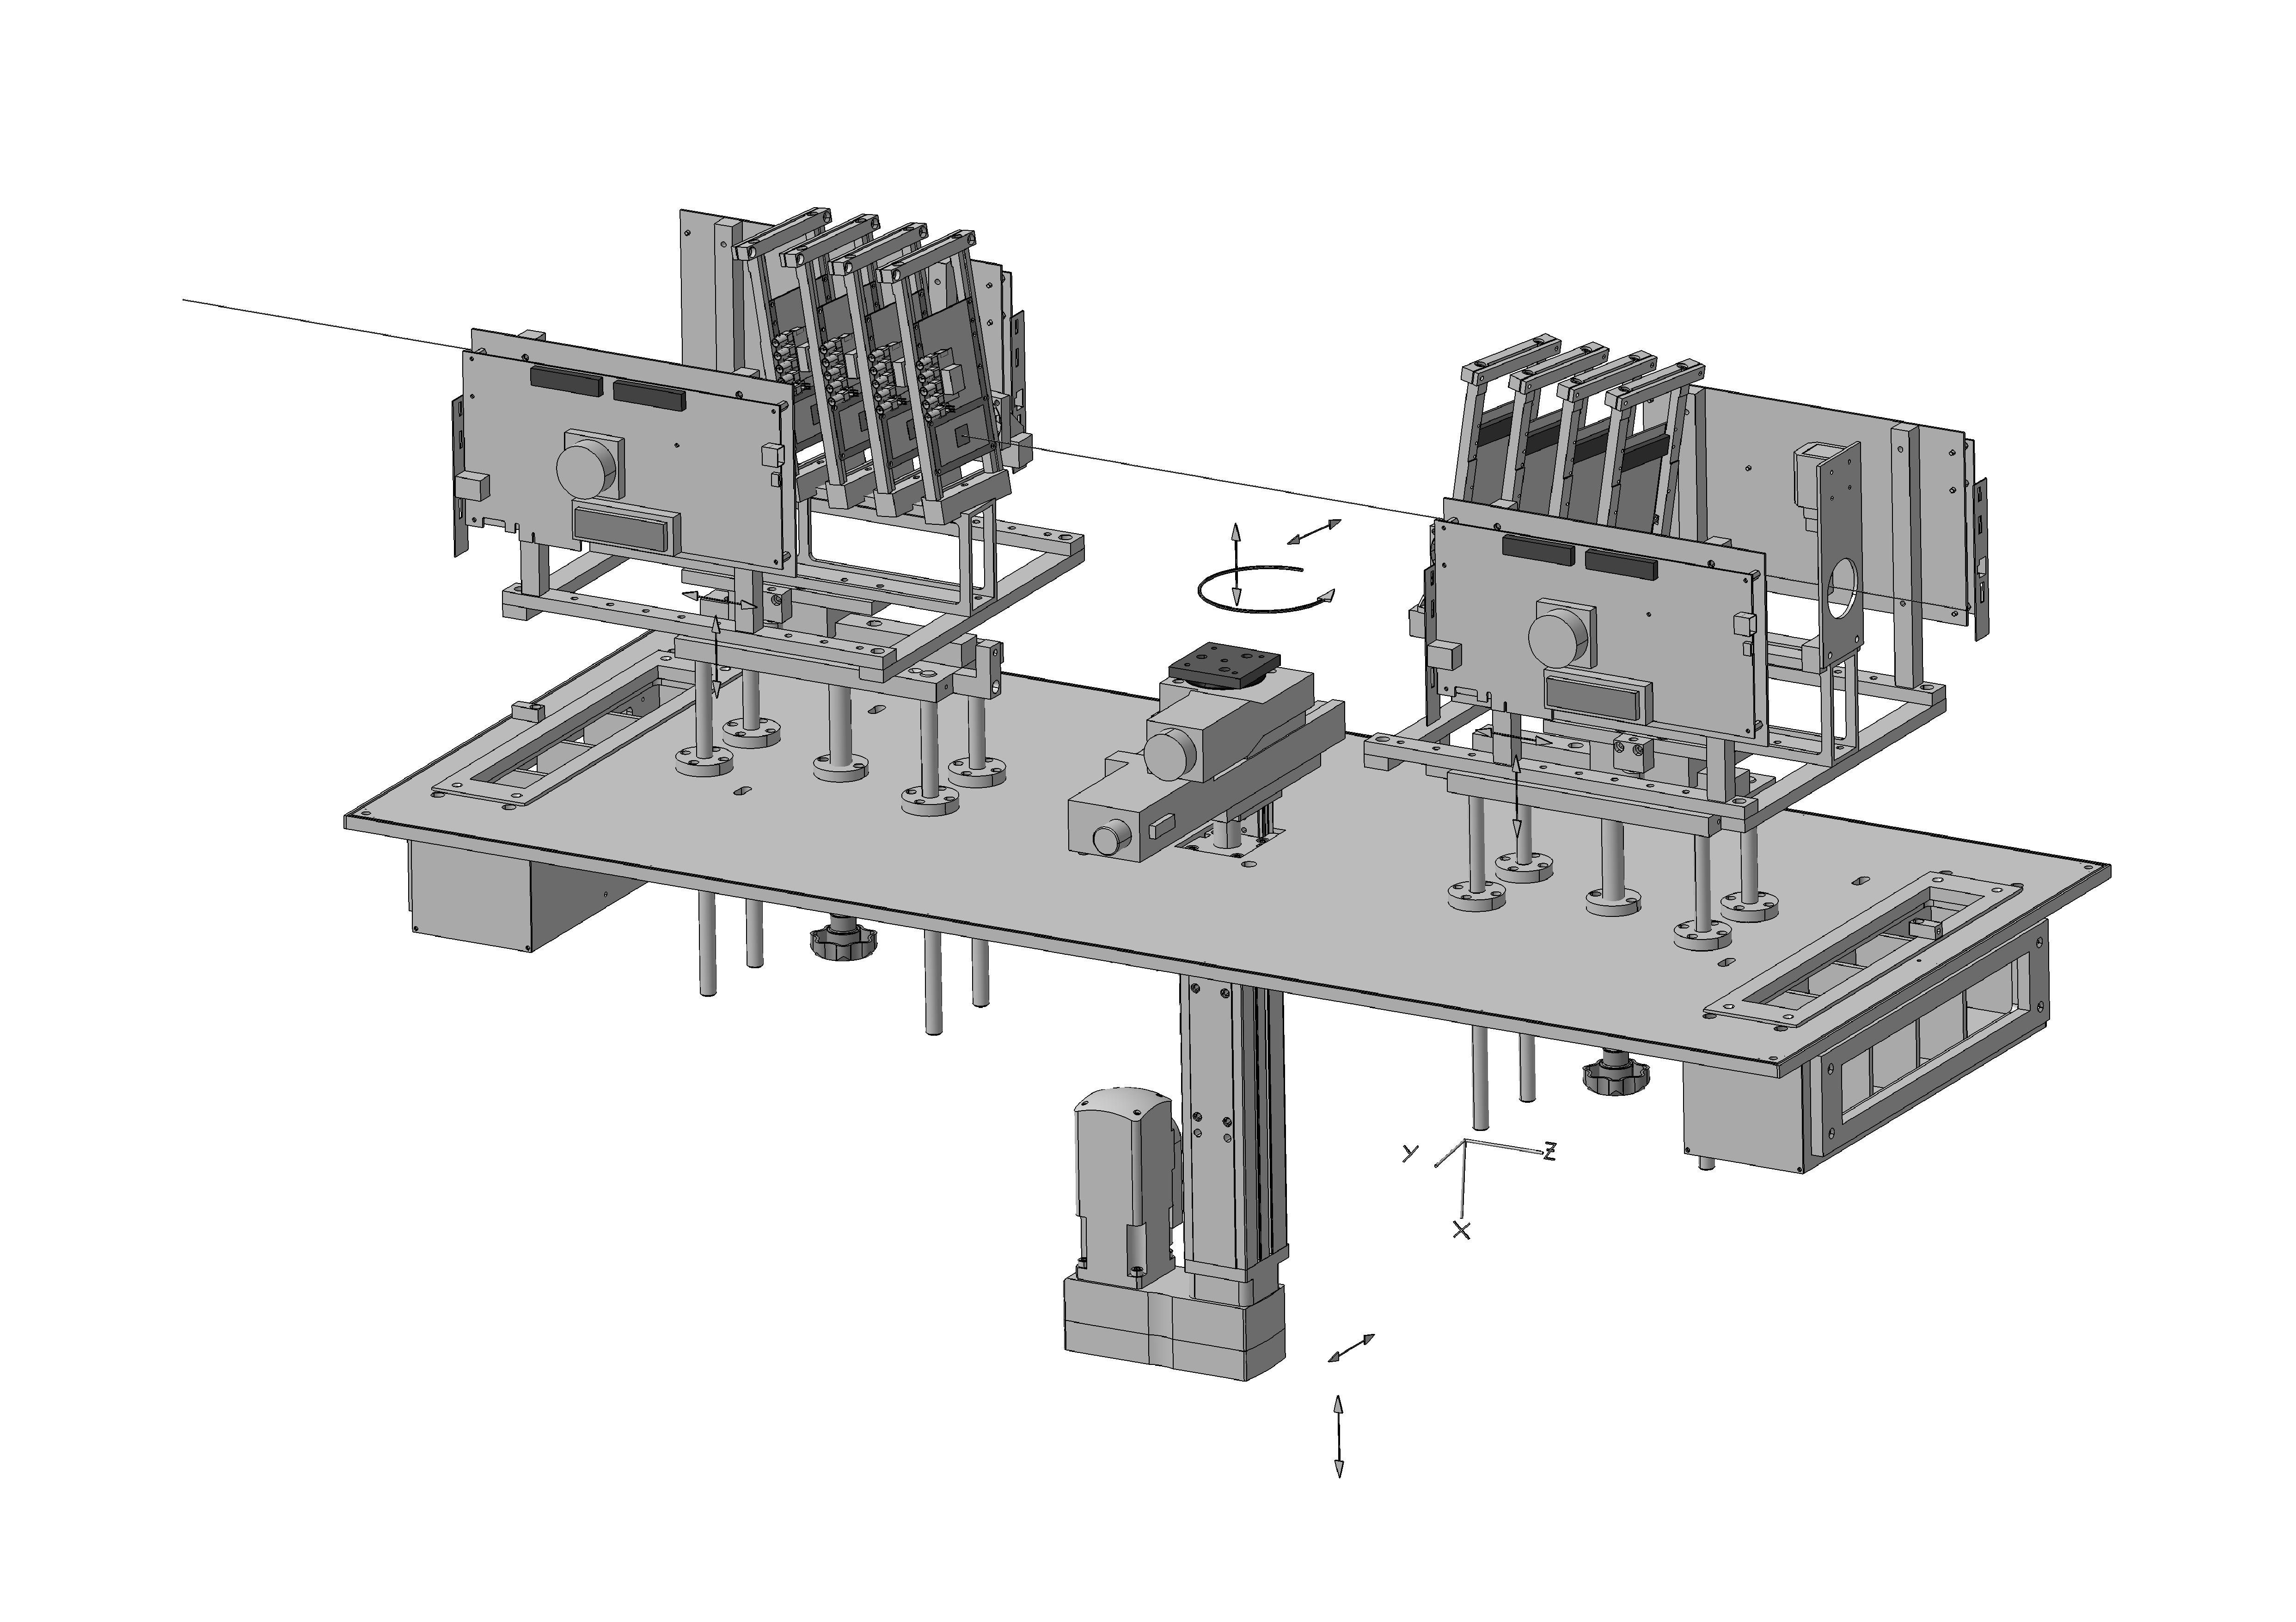
\includegraphics[width=0.7\textwidth]{figs/TelescopeNew.pdf}
\caption[Layout of the Timepix3 telescope.]{Layout of the Timepix3 telescope.}
\label{fig:Telescope}
\end{figure}